\section{ЗАО <<ПКК Миландр>>}

Компания <<Миландр>> выпускает МК для спецприменений,
и (относительно) дешевые варианты МК в пластиковом корпусе для обучения
и неответственных применений.

\bigskip

\begin{tabular}{l l}
Телефон:& (495) 981-54-33 (8.30-17.00, отдел маркетинга и продаж *)\\
Факс:& (495) 981-54-36\\
E-mail:& \email{info@milandr.ru}\\
Сайт:& \url{http://www.milandr.ru}\\
Форум:& \url{http://forum.milandr.ru}\\
Адрес:& 124498, г. Москва, Зеленоград, проезд 4806, дом 6\\
\end{tabular}

\subsection{КР1986ВЕ9х /\cm{3}/}

\begin{wrapfigure}{r}{0.3\textwidth}
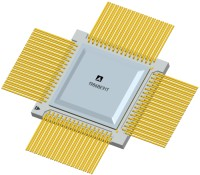
\includegraphics[width=0.3\textwidth]{fig/1986BE94.jpg}
\end{wrapfigure}

\bigskip
\begin{tabular}{l l}
Аналог & STM32F103x\ref{stm32f1}\\
ROM (Flash) & 128K \\
RAM & 32K \\
VCC & $2.2\div3.6$ V\\
Freq & 80 MHz \\
$T^o$ & $-60\div+125$\celsius \\
USB & client/host (12 MBit/s) \\
UART & 2\\
CAN & 2\\
ADC & 2x 12bit 1msps\\
DAC & 12bit\\
\end{tabular}

\bigskip

\begin{tabular}{l l l l l l l l l}
& Pins & SPI & $I^{2}C$ & ADC & DAC & CMP & extBUS &исполнение \\
\hline
1986ВЕ91Т &96 &2 &1 &16ch &2 &3 &32bit &ПЗ5,QFP\\
1986ВЕ94Т &96 &2 &1 &16ch &2 &3 &32bit &ПЗ5\\
1986ВЕ92У  &43 &2 &1 &8ch  &1 &2 &8bit &ПЗ5\\
MDR32F9Q2I &   &  &  &     &  &  &     &QFP\\
К1986ВЕ92QI &   &  &  &     &  &  &     &QFP\\
1986ВЕ93Т &30 &1 &  &4ch  &1 &2 & &ПЗ5\\
\end{tabular}

\subsection{1986ВЕ4У /\cm{0}/}

32-разрядный RISC-микроконтроллер с 8-канальным 24-разрядным $\Sigma\Delta$ АЦП

\bigskip
\begin{tabular}{l l}
ROM (Flash) & 128K \\
RAM & 16K \\
VCC & $2.2\div3.6$ V\\
Freq & 36 MHz \\
$T^o$ & $-60\div+125$\celsius, К $0\div 70$\celsius\\
UART & 2\\
ADC & $\Sigma\Delta$ 24bit, 12bit \\
DAC & 12bit\\
\end{tabular}

\bigskip

\begin{tabular}{l l l l l l l l l}
& Pins & SPI & $I^{2}C$ & ADC & DAC & CMP & extBUS &исполнение \\
\hline
1986ВЕ4У &36 &1 & &8/8ch &1 & & &ПЗ5 \\
\end{tabular}

\subsection{1986ВЕ1Т, К1986ВЕ1QI}


